
%\documentclass[12pt,notitlepage,aps,pra,longbibliography,nofootinbib,tightenlines]{revtex4}
%\documentclass[12pt,notitlepage,longbibliography,nofootinbib,tightenlines]{revtex4-1}

\documentclass[12pt]{article}

%\documentclass[12pt,a4]{revtex4}
%\documentclass[12pt]{article}
%\documentclass[11pt, twocolumn]{article}

%\usepackage{epsf}
\usepackage{amsmath}
\usepackage{color}
\usepackage{natbib}
%\usepackage{cite}
\usepackage{fullpage} % uses 20 percent less pages.

\usepackage{framed}
\usepackage{tikz-cd}

\RequirePackage{amsmath}
\RequirePackage{amssymb}
\RequirePackage{amsthm}
%\RequirePackage{algorithmic}
%\RequirePackage{algorithm}
%\RequirePackage{theorem}
%\RequirePackage{eucal}
\RequirePackage{color}
\RequirePackage{xcolor}
\RequirePackage{url}
\RequirePackage{mdwlist}

\RequirePackage[all]{xy}
\CompileMatrices
\RequirePackage{hyperref}
\RequirePackage{graphicx}
%\RequirePackage[dvips]{geometry}

\newtheorem{theorem}{Theorem}
\newtheorem{lemma}{Lemma}

%\renewenvironment{framed}[1][\hsize]{%
%\def\FrameCommand{{\color{red}\vrule width 3pt}\hspace{0pt}\fboxsep=\FrameSep\colorbox{yellow}}%
%\MakeFramed{\hsize#1\advance\hsize-\width\FrameRestore}}
%{\endMakeFramed}

%\renewenvironment{framed}[1][\hsize]{%
%\def\FrameCommand{{\color{red}\vrule width 3pt}\hspace{0pt}\fboxsep=\FrameSep\colorbox{yellow}}%
%\MakeFramed{\hsize0.8\linewidth\advance\hsize-\width\FrameRestore}}
%{\endMakeFramed}

\renewenvironment{framed}[1][\hsize]{%
\def\FrameCommand{{\color{black}\vrule width 3pt}\hspace{0pt}\fboxsep=\FrameSep\colorbox{lightgray}}%
\MakeFramed{\hsize0.8\linewidth\advance\hsize-\width\FrameRestore}}
{\endMakeFramed}


\begin{document}

\title{Notes on Hecke algebras and more}

\author{Simon Burton}
%\affiliation{Centre for Engineered Quantum Systems, School of Physics, The University of Sydney}

\date{\today}

%\begin{abstract}
%\end{abstract}

\maketitle

%\begin{abstract}
%\end{abstract}

%\newpage
%\tableofcontents
%\newpage

% CUT HERE

\def\Complex{\mathbb{C}}
\def\C{\mathbb{C}}
\def\R{\mathbb{R}}
\def\Z{\mathbb{Z}}
%\def\Ham{\mathcal{H}} % meh..
\def\Ham{H} 
\def\Pauli{\mathcal{P}}
\def\Spec{\mbox{Spec}}
\def\Proveit{{\it (Proof??)}}
\def\GL{\mathrm{GL}}
\def\half{\frac{1}{2}}
\def\Im{\mbox{im}}
\def\Ker{\mbox{ker}}
\def\Field{\mathcal{F}}
\def\Defn#1{\underline{#1}}

\newcommand{\ket}[1]{|{#1}\rangle}
\newcommand{\expect}[1]{\langle{#1}\rangle}
\newcommand{\bra}[1]{\langle{#1}|}
\newcommand{\ketbra}[2]{\ket{#1}\!\bra{#2}}
\newcommand{\braket}[2]{\langle{#1}|{#2}\rangle}


%%%%%%%%%%%%%%%%%%%%%%%%%%%%%%%%%%%%%%%%%%%%%%%%%%%%%%%%%%%%%%%%%%%%%%%%%%%%%%%
%
%%%%%%%%%%%%%%%%%%%%%%%%%%%%%%%%%%%%%%%%%%%%%%%%%%%%%%%%%%%%%%%%%%%%%%%%%%%%%%%
%

\section{Hecke Algebras}

A \Defn{Coxeter group}
has generators $\{s_1, .. s_n \}$
with relations
\begin{align*}
    s_i^2 &= 1 \ \ \mbox{for}\ i=1,..,n\\
    (s_i s_j)^{m(i,j)} &= 1\ \ \mbox{for}\ i,j=1,..,n.
\end{align*}
where $m(i,j)\in\{2,3,4,6\}.$
See \cite{Garrett1997}, \cite{Baez2010}.
A \Defn{dihedral group}
is a Coxeter group with two generators.

The \Defn{Dynkin diagram} (or Coxeter diagram)
associated to a Coxeter group is an undirected graph
with vertices $1,..,n$ and edges $(i,j)$ when $m(i,j)\ge 3.$
The edges are labelled with the value $m(i,j)$.

The \Defn{Hecke algebra} associated with a Dynkin diagram $D$
and $q\ne 0$ 
is the associative algebra $H(D,q)$ with
generators $\sigma_i,\ i=1,..,n$ and relations
\begin{align*}
\sigma_i^2 &= (q-1)\sigma_i + q \\
\sigma_i \sigma_j &= \sigma_j \sigma_i \ \mbox{if}\ m(i,j)=2 \\
\sigma_i \sigma_j \sigma_i &= \sigma_j \sigma_i \sigma_j \ \mbox{if}\ m(i,j)=3 \\
(\sigma_i \sigma_j)^2 &= (\sigma_j \sigma_i)^2 \ \mbox{if}\ m(i,j)=4 \\
(\sigma_i \sigma_j)^3 &= (\sigma_j \sigma_i)^3 \ \mbox{if}\ m(i,j)=6.
\end{align*}
Note that for $m(i,j)=3$ this gives a Yang-Baxter equation and this
explains the connection to knot-theory in such cases (these are the $A_k$ Dynkin diagrams.)

We can factorize the first relation as
$$
    (\sigma_i - q)(\sigma_i + 1) = 0, \ \ i=1,..,n.
$$

The $n$-qubit (real) \Defn{Pauli group} is defined with
$2n$ generators $\{X_i, Z_i\}_{i=1,..,n}$
and relations
\begin{align*}
    X_i^2 = 1,       \ Z_i^2 = 1,\ \ i=1,..,n\\
    (X_i X_j)^2 = 1, \ (Z_i Z_j)^2 = 1,\ \ i,j=1,..,n\\
    (X_i Z_j)^2 = 1, \ (X_i Z_i)^4 = 1, \ i\ne j,\ i,j=1,..,n.
\end{align*}
It follows that this group is an example of a Coxeter group,
but building a Hecke algebra as above will not yield a 
Yang-Baxter equation.


Given a group $G$ and subgroups $H, K$ a
\Defn{double coset}
is the set $HgK=\{hgk | h\in H, k\in K\}.$
The set of double cosets is written $H\backslash G/K.$

%We have an equivelance relation on $G$ given by
%$$
%    g \sim g' \mbox{if} 
%$$
%
%Each double coset $HgK$ is an equivelance class

The group $H\times K$ acts on $G:$ 
$$
    (h, k) : g \mapsto hgk^{-1}.
$$
And the orbits of this action are the double cosets $HgK.$

We can define a \Defn{double coset graph} as follows.
Let $G$ be a group, and $H$ a subgroup of $G.$
Choose $a\in G$ with $a^2\in H.$
We define a graph $\Gamma$
with vertices and edges as
\begin{align*}
    \mbox{V}(\Gamma) &= \{ Hg | g\in G\} \\
    \mbox{E}(\Gamma) &= \{ \{Hx, Hy\} | xy^{-1}\in HaH\}.
\end{align*}
Then $G$ acts on this graph by right multiplication.
This action is vertex-transitive with vertex stabiliser
$$
G_H = \{g \in G | Hg = H\} = H
$$
which acts
transitively on the neighbours $Hah$ (for $h \in H$) of $H$.
Thus $\Gamma$ is arc-transitive \cite{Sabidussi1964}.


\cite{Kassel2010}
exercise 4.2.3: The Hecke algebra of $\GL_n(\Field_q).$

%
% Bruhat decomposition:
% http://mathoverflow.net/questions/15438/a-slick-proof-of-the-bruhat-decomposition-for-gl-nk
%

\subsection{Dynkin diagrams}

\begin{center}
  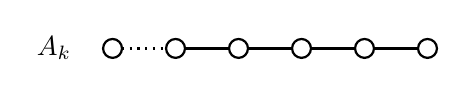
\begin{tikzpicture}[scale=.4]
    \draw (-1,0) node[anchor=east]  {$A_k$};
    \foreach \x in {0,...,5}
    \draw[xshift=\x cm,thick] (\x cm,0) circle (.3cm);
    \draw[dotted,thick] (0.3 cm,0) -- +(1.4 cm,0);
    \foreach \y in {1.15,...,4.15}
    \draw[xshift=\y cm,thick] (\y cm,0) -- +(1.4 cm,0);
  \end{tikzpicture}
\end{center}

\begin{center}
  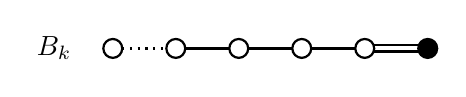
\begin{tikzpicture}[scale=.4]
    \draw (-1,0) node[anchor=east]  {$B_k$};
    \foreach \x in {0,...,4}
    \draw[xshift=\x cm,thick] (\x cm,0) circle (.3cm);
    \draw[xshift=5 cm,thick,fill=black] (5 cm, 0) circle (.3 cm);
    \draw[dotted,thick] (0.3 cm,0) -- +(1.4 cm,0);
    \foreach \y in {1.15,...,3.15}
    \draw[xshift=\y cm,thick] (\y cm,0) -- +(1.4 cm,0);
    \draw[thick] (8.3 cm, .1 cm) -- +(1.4 cm,0);
    \draw[thick] (8.3 cm, -.1 cm) -- +(1.4 cm,0);
  \end{tikzpicture}
\end{center}

\begin{center}
  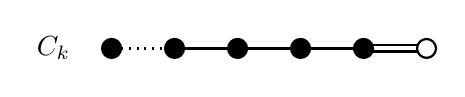
\begin{tikzpicture}[scale=.4]
    \draw (-1,0) node[anchor=east]  {$C_k$};
    \foreach \x in {0,...,4}
    \draw[xshift=\x cm,thick,fill=black] (\x cm,0) circle (.3cm);
    \draw[xshift=5 cm,thick] (5 cm, 0) circle (.3 cm);
    \draw[dotted,thick] (0.3 cm,0) -- +(1.4 cm,0);
    \foreach \y in {1.15,...,3.15}
    \draw[xshift=\y cm,thick] (\y cm,0) -- +(1.4 cm,0);
    \draw[thick] (8.3 cm, .1 cm) -- +(1.4 cm,0);
    \draw[thick] (8.3 cm, -.1 cm) -- +(1.4 cm,0);
  \end{tikzpicture}
\end{center}

\begin{center}
  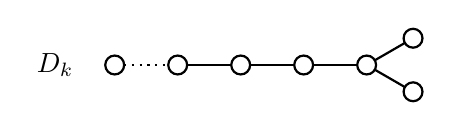
\begin{tikzpicture}[scale=.4]
    \draw (-1,0) node[anchor=east]  {$D_k$};
    \foreach \x in {0,...,4}
    \draw[xshift=\x cm,thick] (\x cm,0) circle (.3cm);
    \draw[xshift=8 cm,thick] (30: 17 mm) circle (.3cm);
    \draw[xshift=8 cm,thick] (-30: 17 mm) circle (.3cm);
    \draw[dotted,thick] (0.3 cm,0) -- +(1.4 cm,0);
    \foreach \y in {1.15,...,3.15}
    \draw[xshift=\y cm,thick] (\y cm,0) -- +(1.4 cm,0);
    \draw[xshift=8 cm,thick] (30: 3 mm) -- (30: 14 mm);
    \draw[xshift=8 cm,thick] (-30: 3 mm) -- (-30: 14 mm);
  \end{tikzpicture}
\end{center}

\begin{center}
  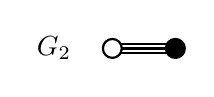
\begin{tikzpicture}[scale=.4]
    \draw (-1,0) node[anchor=east]  {$G_2$};
    \draw[thick] (0 ,0) circle (.3 cm);
    \draw[thick,fill=black] (2 cm,0) circle (.3 cm);
    \draw[thick] (30: 3mm) -- +(1.5 cm, 0);
    \draw[thick] (0: 3 mm) -- +(1.4 cm, 0);
    \draw[thick] (-30: 3 mm) -- +(1.5 cm, 0);
  \end{tikzpicture}
\end{center}

\begin{center}
  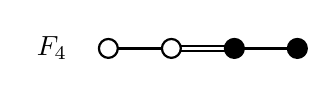
\begin{tikzpicture}[scale=.4]
    \draw (-3,0) node[anchor=east]  {$F_4$};
    \draw[thick] (-2 cm ,0) circle (.3 cm);
    \draw[thick] (0 ,0) circle (.3 cm);
    \draw[thick,fill=black] (2 cm,0) circle (.3 cm);
    \draw[thick,fill=black] (4 cm,0) circle (.3 cm);
    \draw[thick] (15: 3mm) -- +(1.5 cm, 0);
    \draw[xshift=-2 cm,thick] (0: 3 mm) -- +(1.4 cm, 0);
    \draw[thick] (-15: 3 mm) -- +(1.5 cm, 0);
    \draw[xshift=2 cm,thick] (0: 3 mm) -- +(1.4 cm, 0);
  \end{tikzpicture}
\end{center}

\begin{center}
  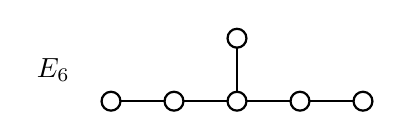
\begin{tikzpicture}[scale=.4]
    \draw (-1,1) node[anchor=east]  {$E_6$};
    \foreach \x in {0,...,4}
    \draw[thick,xshift=\x cm] (\x cm,0) circle (3 mm);
    \foreach \y in {0,...,3}
    \draw[thick,xshift=\y cm] (\y cm,0) ++(.3 cm, 0) -- +(14 mm,0);
    \draw[thick] (4 cm,2 cm) circle (3 mm);
    \draw[thick] (4 cm, 3mm) -- +(0, 1.4 cm);
  \end{tikzpicture}
\end{center}

\begin{center}
  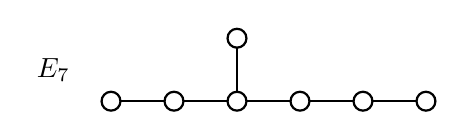
\begin{tikzpicture}[scale=.4]
    \draw (-1,1) node[anchor=east]  {$E_7$};
    \foreach \x in {0,...,5}
    \draw[thick,xshift=\x cm] (\x cm,0) circle (3 mm);
    \foreach \y in {0,...,4}
    \draw[thick,xshift=\y cm] (\y cm,0) ++(.3 cm, 0) -- +(14 mm,0);
    \draw[thick] (4 cm,2 cm) circle (3 mm);
    \draw[thick] (4 cm, 3mm) -- +(0, 1.4 cm);
  \end{tikzpicture}
\end{center}

\begin{center}
  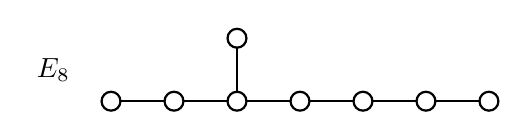
\begin{tikzpicture}[scale=.4]
    \draw (-1,1) node[anchor=east]  {$E_8$};
    \foreach \x in {0,...,6}
    \draw[thick,xshift=\x cm] (\x cm,0) circle (3 mm);
    \foreach \y in {0,...,5}
    \draw[thick,xshift=\y cm] (\y cm,0) ++(.3 cm, 0) -- +(14 mm,0);
    \draw[thick] (4 cm,2 cm) circle (3 mm);
    \draw[thick] (4 cm, 3mm) -- +(0, 1.4 cm);
  \end{tikzpicture}
\end{center}


%%%%%%%%%%%%%%%%%%%%%%%%%%%%%%%%%%%%%%%%%%%%%%%%%%%%%%%%%%%%%%%%%%%%%%%%%%%%%%%
%
%%%%%%%%%%%%%%%%%%%%%%%%%%%%%%%%%%%%%%%%%%%%%%%%%%%%%%%%%%%%%%%%%%%%%%%%%%%%%%%
%

\section{Discrete differential geometry}

Regge calculus aka Discrete exterior calculus.
Applications to building space-time geometry out of
quantum entanglement structures: \cite{Cao2016}.
Constructing a Ricci flow on a simplicial geometry: \cite{Miller2014}.


%%%%%%%%%%%%%%%%%%%%%%%%%%%%%%%%%%%%%%%%%%%%%%%%%%%%%%%%%%%%%%%%%%%%%%%%%%%%%%%
%
%%%%%%%%%%%%%%%%%%%%%%%%%%%%%%%%%%%%%%%%%%%%%%%%%%%%%%%%%%%%%%%%%%%%%%%%%%%%%%%
%

\section{ADE classification}

Singularities:
\begin{align*}
A_k:f(x)   &= x^{k+1}, \ \ k\ge 1;\\
D_k:f(x,y) &= x^2y + y^{k-1},\ \  k\ge 4;\\
E_6:f(x,y) &= x^3 + y^4;\\
E_7:f(x,y) &= x^3 + xy^3;\\
E_8:f(x,y) &= x^3 + y^5.
\end{align*}

Platonic solid symmetry:
$E_6:$ tetrahedral, $E_7:$ cube (octahedral), $E_8:$ icosahedron (dodecahedron.)

Another trinity: Real, Complex, Quaternionic.

The $ADE$ Dynkin diagrams are the simply laced diagrams (single edges only.)

% http://blogs.ams.org/visualinsight/2016/05/01/involutes-of-a-cubical-parabola/

% https://en.wikipedia.org/wiki/Catastrophe_theory#Elementary_catastrophes



%%%%%%%%%%%%%%%%%%%%%%%%%%%%%%%%%%%%%%%%%%%%%%%%%%%%%%%%%%%%%%%%%%%%%%%%%%%%%%%
%
%%%%%%%%%%%%%%%%%%%%%%%%%%%%%%%%%%%%%%%%%%%%%%%%%%%%%%%%%%%%%%%%%%%%%%%%%%%%%%%
%

\section{Higher structures}

% http://chocolatshalba.ch/files/texlive/texmf-dist/doc/latex/tikz-cd/tikz-cd-doc.pdf

A \Defn{groupoid} is a category where every morphism is invertible.

Given a group $G$ acting on a set $X$
the \Defn{weak quotient} $X//G$
is the groupoid with objects $X$ and morphisms
\[\begin{tikzcd} x \arrow{r}{g} & gx \end{tikzcd} \]

The groupoid $G//G$ has morphisms that look like
\[\begin{tikzcd} g \arrow{r}{h} & hg \end{tikzcd} \]
for $g, h\in G.$
This also has a monoidal structure; given two
morphisms
\[\begin{tikzcd}[row sep=small]
g_1 \arrow{r}{h_1} & h_1g_1 \\
g_2 \arrow{r}{h_2} & h_2g_2
\end{tikzcd} \]
we form
\[\begin{tikzcd}[row sep=large, column sep = large]
g_2 g_1 \arrow{r}{h_2 g_2 h_1 g_2^{-1}} & h_2 g_2 h_1 g_1 
\end{tikzcd} \]
The monoidal product has an inverse: 
each morphism 
$$h:g\to hg$$ 
has inverse 
$$g^{-1}hg : g^{-1}\to (hg)^{-1}.$$
This makes $G//G$ into a strict 2-Group \cite{Roberts2007}.

\def\bdy{\partial}

Changing notation now, we take as our group a vector space $m,$
then for $v,v'\in m$ we have the morphism
\[\begin{tikzcd}[column sep = large]
v \arrow{r}{v'-v} & v'. \end{tikzcd} \]
We can extend this idea to a 2-groupoid as follows.
%strict symmetric monoidal 3-groupoid ?
Given a linear operator $\bdy$
\[\begin{tikzcd} 0 \arrow{r} & m_2 \arrow{r}{\bdy} & m_1 \arrow{r} & 0 \end{tikzcd} \]
is a groupoid with objects $m_1$ and
for $v_1, v_1'\in m_1$ with $v_1'-v_1 \in \Im(\bdy)$
we have morphisms
\[\begin{tikzcd}[column sep = large]
v_1 \arrow{r}{v_2} & v_1'. \end{tikzcd} \]
with $\bdy v_2=v_1'-v_1.$
Given two such morphisms $v_2, v'_2$ with $\bdy v_2=\bdy v_2'=v_1'-v_1$ 
we get a 2-morphism $u_2=v_2'-v_2\in\Ker(\bdy)$:
$$
\begin{tikzcd}[column sep = small, row sep = tiny]
\ \arrow{rr}[]{v_2} \arrow{rr}[name=U,below]{} & \ & \   \\
v_1         & \ \ \ \ {}_{u_2}              & v_1' \\
\ \arrow{rr}[below]{v_2'} \arrow{rr}[name=D]{}  &  \     & \   \\
\arrow[Rightarrow,to path=(U) -- (D),left]{}
\end{tikzcd}
$$

Bumping up a dimension we get to
\[\begin{tikzcd} 0 \arrow{r} & m_3 \arrow{r}{\bdy_3} & m_2 \arrow{r}{\bdy_2} & m_1 \arrow{r} & 0 \end{tikzcd} \]
and now if we have 2-morphisms $u_2, u'_2: v_2 \to v'_2 $
such that $u'_2-u_2\in \Im(\bdy_3)$
we have a 3-morphism $u_3:u_2\to u'_2$ 
given by an element $u_3\in m_3$ such that $\bdy(u_3)=u'_2-u_2:$
$$
\begin{tikzcd}[column sep = tiny, row sep = tiny]
\ \arrow{rrr}[]{v_2} \arrow{rrr}[pos=0.3,name=U,below]{} \arrow{rrr}[pos=0.7,name=UU,below]{} & \ & \ &\  \\
v_1         & {}_{u_2} \ \ \ \ \ \overset{u_3}{\Rrightarrow} & {}_{u'_2}    & v_1' \\
\ \arrow{rrr}[below]{v_2'} \arrow{rrr}[pos=0.3,name=D]{} \arrow{rrr}[pos=0.7,name=DD]{}   &  \   &\  & \   \\
\arrow[Rightarrow,to path=(U) -- (D),left]{}
\arrow[Rightarrow,to path=(UU) -- (DD),left]{}
\end{tikzcd}
$$
% another globular pic:
% http://tex.stackexchange.com/questions/157089/drawing-diagrams-of-higher-categories-with-tikz

%$$
%\begin{tikzcd}[column sep = small, row sep = tiny]
%\ \arrow{rrr}[]{v_2} \arrow{rrr}[pos=0.2,name=U,below]{} \arrow{rrr}[pos=0.8,name=UU,below]{} & \ & \ &\  \\
%v_1         & {}_{u_2} \arrow{r}{u_3}     & {}_{u'_2}    & v_1' \\
%\ \arrow{rrr}[below]{v_2'} \arrow{rrr}[pos=0.2,name=D]{} \arrow{rrr}[pos=0.8,name=DD]{}   &  \   &\  & \   \\
%\arrow[Rightarrow,to path=(U) -- (D),left]{}
%\arrow[Rightarrow,to path=(UU) -- (DD),left]{}
%\end{tikzcd}
%$$




%\begin{tikzcd}[column sep = huge]
%A \arrow{r}[name=U,below]{} & B \\
%B \arrow{r}[name=D]{} & C \\
%\arrow[Rightarrow,to path=(U) -- (D)]{}
%\end{tikzcd}
%
%\begin{tikzcd}
%A \arrow[bend left=50]{r}[name=U,below]{}
%\arrow[bend right=50]{r}[name=D]{}
%& B
%\arrow[Rightarrow,to path=(U) -- (D)]{}
%\end{tikzcd}

\subsection{Monads}

A \emph{monad} on a category $\C$ is an endofunctor $T:\C\to \C$
and two natural transformations,
a unit $\eta:1_\C\to T$ and a multiplication $\mu:T^2\to T.$

\[
\begin{tikzcd}
T^3 \arrow{r}{T\mu} \arrow[swap]{d}{\mu T} & T^2 \arrow{d}{\mu} & 
T \arrow{r}{\eta T}\arrow{dr}{=} & T^2 \arrow{d}{\mu} & \arrow[swap]{l}{T\eta}\arrow{dl}{=} T \\
T^2 \arrow{r}{\mu} & T & 
& T & 
\end{tikzcd}
\]

%\[
%\begin{tikzcd}
%A \arrow{r}{f} \arrow[swap]{dr}{g\circ f} & B \arrow{d}{g} \\
%& C
%\end{tikzcd}
%\]

See \cite{Mac1978}, \cite{Jacobs2012}.

The distribution monad relies on the self-distributivity of convexity.
See \cite{Jacobs2012} section 5.1.3.






\bibliography{refs}{}
\bibliographystyle{abbrv}


\end{document}


